\documentclass[12pt,letterpaper]{article}
\usepackage{fullpage}
\usepackage[top=2cm, bottom=4cm, left=2.5cm, right=2.5cm]{geometry}
\usepackage{amsmath,amsthm,amsfonts,amssymb,amscd}
\usepackage{lastpage}
\usepackage{enumerate}
\usepackage{fancyhdr}
\usepackage{mathrsfs}
\usepackage{xcolor}
\usepackage{graphicx}
\usepackage{listings}
\usepackage{hyperref}
\usepackage{float}

\hypersetup{%
  colorlinks=true,
  linkcolor=blue,
  linkbordercolor={0 0 1}
}
 
\renewcommand\lstlistingname{Algorithm}
\renewcommand\lstlistlistingname{Algorithms}
\def\lstlistingautorefname{Alg.}

\lstdefinestyle{Python}{
    language        = Python,
    frame           = lines, 
    basicstyle      = \footnotesize,
    keywordstyle    = \color{blue},
    stringstyle     = \color{green},
    commentstyle    = \color{red}\ttfamily
}

\setlength{\parindent}{0.0in}
\setlength{\parskip}{0.05in}
\begin{document}
    Sunny Lee

    \begin{enumerate}
        \item Running Newton's method: \\
        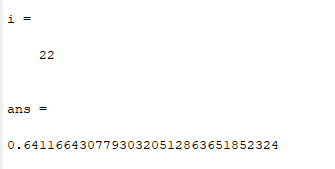
\includegraphics{number1.png}
        \item 
        Running the Modified Newton's method:
        at $p = 0.64116643$. Using the first and second derivative: \\
        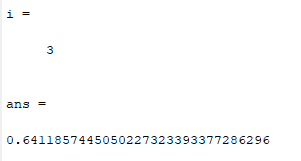
\includegraphics{number2.png}\\
        So we see that the Modified Newton's converges much faster than the regular
        Newton's method. 
        
        \item
        Using Newton's method: \\
        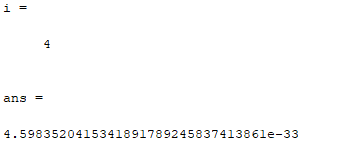
\includegraphics{number3.png}

        \item 
        \begin{enumerate}
            \item 
            Taking the errors for each iteration: \\
            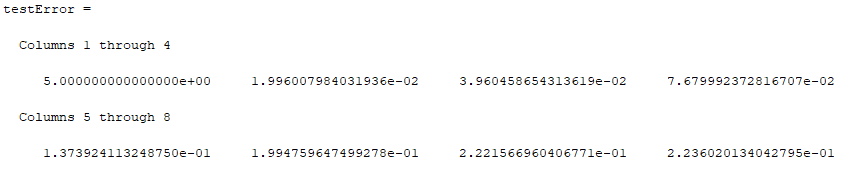
\includegraphics[scale = .7]{number4.png}\\
            Comparing our last value with the actual value of the error:\\
            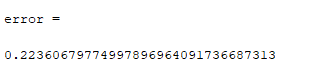
\includegraphics{numbe4error.png}\\
            We see that the test error and the theoretical error are quite close. 

            \item 
            Running the errors on secant method, we find that the asymptotic error constant
            is about $.78510$: \\
            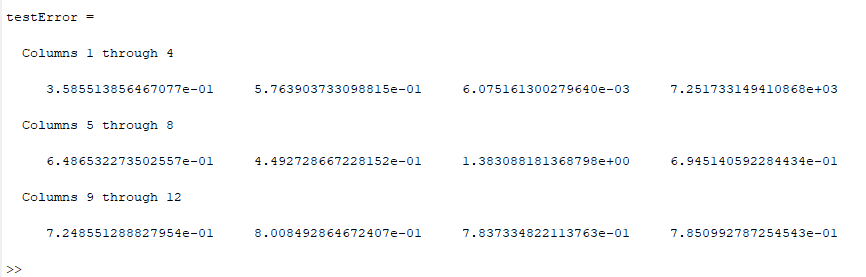
\includegraphics[scale = .7]{number5.png}\\
            We also see from the errors that secant method took more iterations than 
            Newton's method, confirming that secant method has a lower rate of convergence
            than Newton's method. 
        \end{enumerate}

        \item
        \begin{gather*}
            e_{k+1} = x_{k+1} - x^* = g(x_k) - g(x^*)
        \end{gather*}
        Using a Taylor expansion around $x^*$ and evaluated at $x_k$: 
        \begin{gather*}
            g(x_k) \approx g(x^*) + g'(x^*)(x_k - x^*) + \frac{1}{2}g''(x^*)(x_k - x^*)^2 + \frac{1}{6}g^{(3)}(x^*)(x_k - x^*)^3 \\
            + \frac{1}{24}g^{(4)}(c)(x_k - x^*)^4
        \end{gather*}
        Where $c\in [x_k, x^*]$. Since $g'(x^*) = g''(x^*) = g^{(3)}(x^*) = 0$ we can 
        reduce our function to: 
        \begin{gather*}
            g(x_k) - g(x^*) = \frac{1}{24}g^{(4)}(c)(x_k - x^*)^4
        \end{gather*}
        Thus: 
        \begin{gather*}
            e_{k+1} = \frac{1}{24}g^{(4)}(c)e_k^4\\
            \lim_{k\rightarrow \infty} \frac{|e_{k+1}|}{|e_k^4|} = |\frac{1}{24}g^{(4)}(c)|
        \end{gather*}
        Therefore, the order of convergence is $4$, and our asymptotic error constant is 
        $|\frac{1}{24}g^{(4)}(c)|$. 
    \end{enumerate}
\end{document}